\documentclass[12pt,A4]{extarticle}	

\usepackage{amsfonts}
\usepackage{amsmath}
\usepackage{amssymb}
\usepackage{graphicx,wrapfig,lipsum}
\usepackage[german]{babel}

\newcommand{\lectureTitle}{Symmetrische Verschlüsselungsverfahren [WIP]}
\newcommand{\semester}{Sommersemester 2023}

\newcommand{\titleSize}{\LARGE}

\usepackage[a4paper,left=0.9cm,right=1cm,top=1.37cm,bottom=2.5cm]{geometry}
\usepackage[utf8]{inputenc}
\usepackage{xifthen}
\usepackage{cmbright}
\usepackage{fontawesome}
\usepackage[T1]{fontenc}
\usepackage{lastpage,lipsum}
\usepackage{hyperref}
\usepackage{transparent}
\usepackage{color}
\usepackage{fancyhdr}

\renewcommand*\familydefault{\sfdefault}
\setlength{\parindent}{0mm}

\definecolor{headerBg}{RGB}{11, 67, 158}
\definecolor{headerGrayColor}{RGB}{210, 210, 210}

\newcommand{\printTitle}{\textcolor{white}{\lectureTitle}\normalsize}
\newcommand{\printSubtitle}{
  \ifdefined\lectureSubtitle
    \textcolor{white}{\small{\lectureSubtitle}}\\
  \fi
}

\fancyhf{}
\pagestyle{fancy}
\fancyhead[C]{
  \fcolorbox{headerBg}{headerBg}{
    \hspace{0.6cm}\begin{minipage}[c][50pt][c]{\paperwidth}
      \begin{minipage}[c]{.7\textwidth}
        \ifdefined\titleSize
          \titleSize \printTitle\\
        \else
          \huge\printTitle\\
        \fi
        \printSubtitle
        \textcolor{headerGrayColor}{\small{\semester}}
      \end{minipage}%
      \begin{minipage}[c]{.2\textwidth}
        \raggedleft
        \textcolor{white}{
          \small{\href{mailto:mail@nilslambertz.de}{\textcolor{white}{\faicon{envelope}} mail@nilslambertz.de}}\\
          \href{https://github.com/nilslambertz/kit-zusammenfassungen}{\textcolor{white}{\faicon{github}} \small{nilslambertz}}}
      \end{minipage}
    \end{minipage}}
}
\renewcommand{\headrulewidth}{0pt}
\setlength{\headheight}{40pt}

\newlength{\oddmarginwidth}
\setlength{\oddmarginwidth}{1in+\hoffset+\oddsidemargin}
\newlength{\evenmarginwidth}
\setlength{\evenmarginwidth}{\evensidemargin+1in}
\fancyhfoffset[LO,RE]{\oddmarginwidth}
\fancyhfoffset[LE,RO]{\evenmarginwidth}
\cfoot{\thepage\ $/$ \pageref*{LastPage}}

\definecolor{highlightColor}{RGB}{66, 135, 245}
\newcommand{\highlight}[1]{\textcolor{highlightColor}{\textbf{#1}}}

\newcommand{\redBold}[1]{\textcolor{red}{\textbf{#1}}}

\def\contentsname{\empty}
\addto\captionsgerman{
  \renewcommand{\contentsname}{\empty}
}

\begin{document}

\disclaimer

\tableofcontents
\clearpage

\section{Einführung}
\subsection{Ausgangspunkte für Angriffe}
Angriffe können nach den zur Verfügung stehenden Informationen unterteilt werden:
\begin{itemize}
  \item{\highlight{Ciphertext-Only-Attack}: Nur das \textit{Chiffre}, also die verschlüsselte Nachricht, ist bekannt}
  \item{\highlight{Known-Plaintext-Attack}: Es gibt bekannte Klartext-Chiffre-Paare. Hilfreich sind bekannte Anfangs- und Endphrasen, die in mehreren Nachrichten vorkommen.}
  \item{\highlight{Chosen-Plaintext-Attack}: Es besteht die Möglichkeit, beliebige Texte zu verschlüsseln und somit Klartext-Chiffre-Paare zu erzeugen.}
\end{itemize}

\subsection{Angriffsarten}
\begin{itemize}
  \item{Brute-Force (z.B. alle Schlüssel ausprobieren)}
  \item{Statistische Methoden (z.B. Häufigkeitsanalysen von Buchstaben)}
  \item{Strukturelle Angriffe (z.B. Lineare Kryptoanalyse)}
\end{itemize}

\subsection{Historische Verschlüsselungsverfahren}
Historisch wurden zur Verschlüsselung zwei grundlegende Operationen verwendet:
\begin{itemize}
  \item{\highlight{Substitution}}
  \item{\highlight{Permutation}}
\end{itemize}
Alleine sind beide Verfahren meistens nicht sicher, jedoch verwenden moderne Verschlüsselungsverfahren eine Kombination beider Operationen.

\section{Blockchiffren}
\subsection{Definitionen}
\subsubsection{Definition: Blockchiffre}
Gegeben seien zwei endliche Alphabete $A, B$ und $n, m \in \mathbb{N}$ sowie ein Schlüsselraum $\mathcal{K}$. Eine \highlight{Blockchiffre} ist gegeben durch eine Familie von injektiven Abbildungen $f_k: A^n \rightarrow B^m$ mit $k \in \mathcal{K}$. In der Regel gilt $A = B = \{0, 1\}$ und $n = m$.

\subsubsection{Anforderungen an Blockchiffren}
\begin{itemize}
  \item{Gegeben den Schlüssel $k$ müssen sowohl $f_k$ als auch $f^{-1}_k$ \textbf{effizient} berechenbar sein}
  \item{Ein Angreifer soll nicht zwischen einer \textit{zufälligen Abbildung} und der Blockchiffre mit \textit{zufälligem Schlüssel} unterscheiden können}
\end{itemize}

\subsubsection{Definition: Ideal Cipher}
Eine \highlight{Ideal Cipher} (IC) ist eine (Über-)Idealisierung einer Blockchiffre. Jedem Schlüssel $k \in \{0, 1\}^\lambda$ ist eine vollkommen zufällige Permutation $P_k: \{0, 1\}^n \rightarrow \{0, 1\}^n$ zugeordnet (hierbei sind $\lambda$ und $n$ Sicherheitsparameter) und per Orakelzugriff kann jede Maschine im Modell die Funktionen $P_k$ und $P^{-1}_k$ auswerten. Die Existenz einer solchen IC wird zur Vereinfachung von Beweisen angenommen, man spricht dann von dem \textbf{Ideal-Cipher-Modell}.

\subsubsection{Anforderungen an Ideal Cipher}
\begin{itemize}
  \item{Alle Parteien können über Orakelzugriff $P_k$ und $P^{-1}_k$ auswerten}
  \item{Ideal Cipher liefert zu jedem Paar $(k, m)$ ein $c$ ``zufällig'' gewählt}
  \item{Ideal Cipher liefert zu jedem Paar $(k, c)$ ein $m$ ``zufällig'' gewählt}
  \item{Orakel muss jede Ausgabe speichern, damit für gleiche Nachrichten immer das gleiche Chiffre zurückgegeben wird (nicht parallelisierbar)}
\end{itemize}

\begin{wrapfigure}{r}{9cm}
  \vspace*{-2cm}
  \centering
  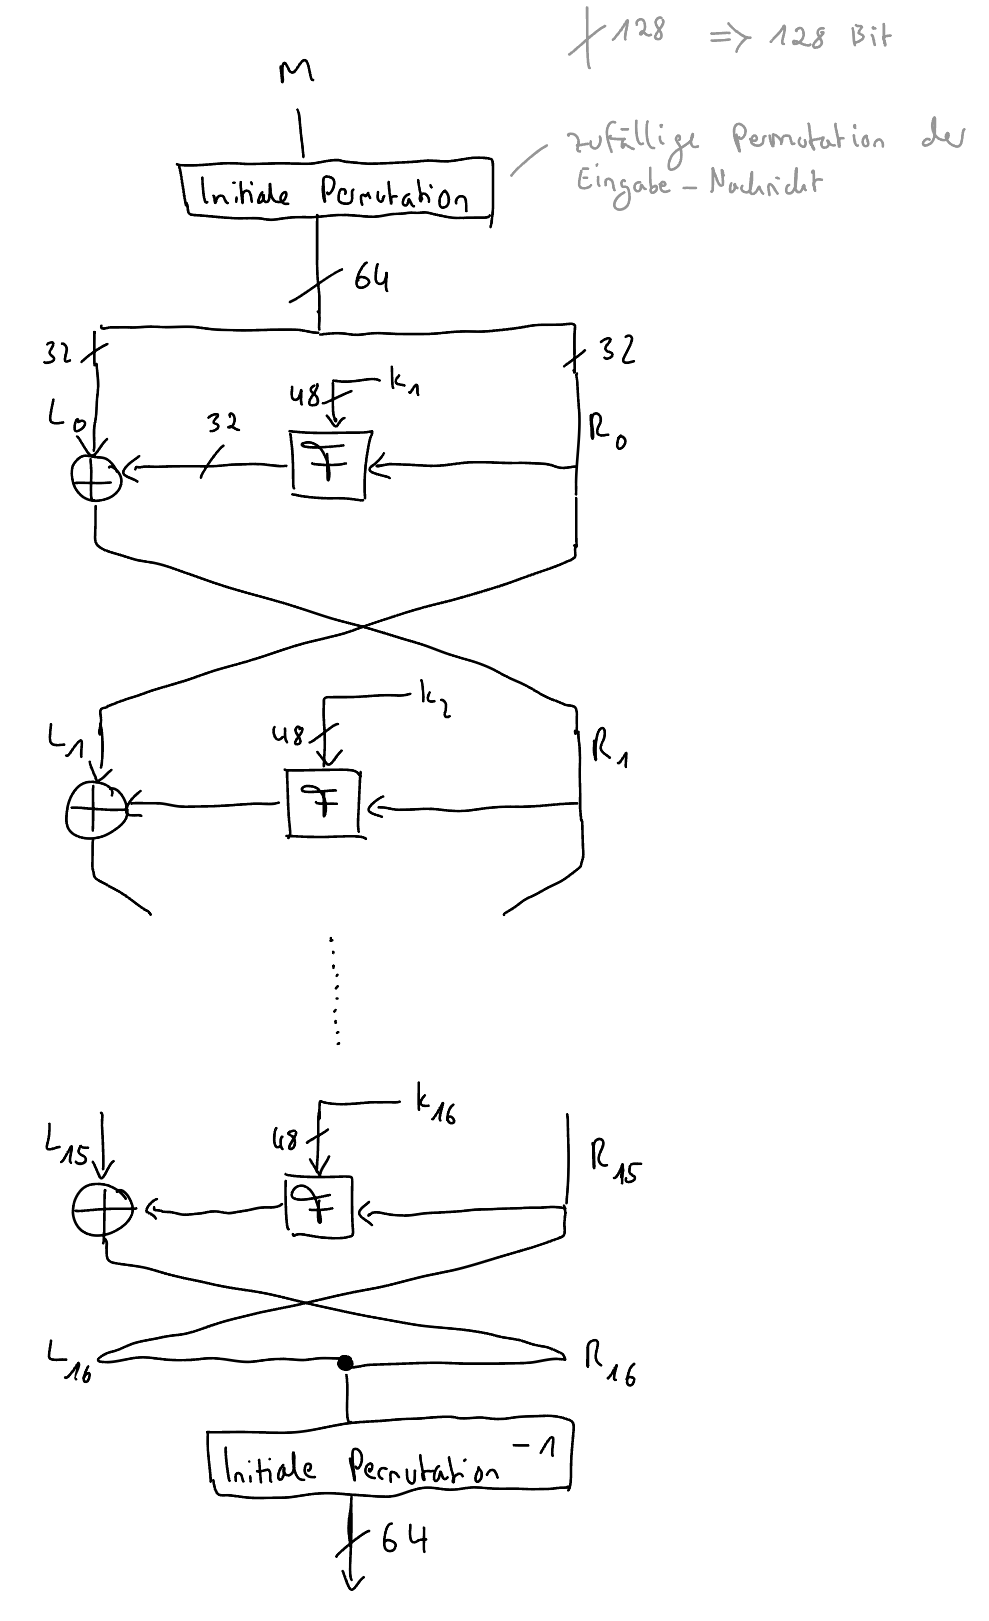
\includegraphics[width=8cm]{../images/des_struktur.png}
  \caption{DES-Verschlüsselungsalgorithmus}
  \vspace*{0.5cm}
  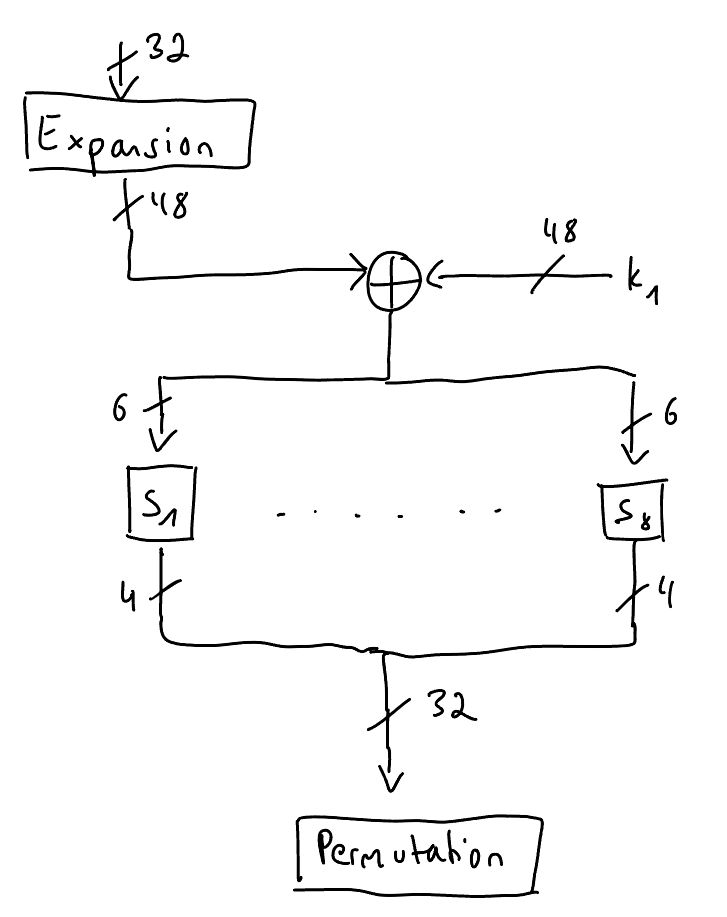
\includegraphics[width=6cm]{../images/des_f_funktion.png}
  \caption{F-Funktion}
  \vspace*{-10cm}
\end{wrapfigure}
\subsection{DES (Data Encryption Standard)}
Der \textbf{Data Encryption Standard} ist eine Blockchiffre mit Schlüssellänge $k = 56$ und Blocklänge $n = 64$, die Verschlüsselungsfunktion ist also $\{0, 1\}^k \times \{0, 1\}^n \rightarrow \{0, 1\}^n$. Er besteht aus einer \textbf{Feistel-Struktur} mit 16 Runden und wurden aufgrund der kurzen Schlüssellänge \textbf{gebrochen}.
\subsubsection{Beispiel für Encryption-Schritt}
$L_1 = R_0$\\
$R_1 = L_0 \oplus F_{k_1}(R_0)$\par
$L_{16} = R_{15}$\\
$R_{16} = L_{15} \oplus F_{k_{16}}(R_{15})$\par

\subsubsection{Beispiel für Decryption-Schritt}
$R_{15} = L_{16}$
\begin{flalign*}
  L_{15} & = R_{16} \oplus F_{k_{16}}(R_{15}) & \\
         & = R_{16} \oplus F_{k_{16}}(L_{16})
\end{flalign*}

\subsubsection{F-Funktion}
Die \highlight{F-Funktion} ist eine nicht-reversible Funktion, die in jeder Runde der Feistel-Struktur ausgeführt wird. Der Ablauf ist folgender:
\begin{enumerate}
  \item{\textbf{Expansion}: Die 32 Eingabebits werden auf 48 Bits erweitert}
  \item{Das bitweise XOR zwischen Expansion und dem Schlüssel wird berechnet}
  \item{Das Ergebnis wird in 6-Bit-Blöcken auf 8 \textbf{Substitutionsboxen} verteilt}
  \item{Die Substitution wird permutiert und ausgeben}
\end{enumerate}

\newpage
\subsection{2DES}\label{sec:2des}
DES wurde aufgrund der kurzen Schlüssellänge (56 Bit) gebrochen und sollte daher nicht mehr in seiner einfachen Form verwendet werden. Es gibt jedoch modifizierte Varianten, die die Sicherheit von DES verbessern, z.B. \textbf{2DES}:\par
Bei 2DES wird die Nachricht zuerst mit $k_1$ verschlüsselt und das Chiffrat dann erneut mit $k_2$ verschlüsselt: $c = DES_{k_2}(DES_{k_1}(m))$

\subsubsection{Angriff auf 2DES}
Gegen 2DES sind \textbf{Meet-in-the-Middle}-Angriffe möglich, dabei wird versucht, die Verschlüsselung von beiden Seiten zu brechen.\par
Gegeben sind zwei Paare $(m_1, c_1)$ und $(m_2, c_2)$, dann funktioniert der Angriff wie folgt:
\begin{enumerate}
  \item{\textbf{Vorwärtsschritt}: Berechne $DES_{k}(m_1)$ und $DES_{k}(m_2)$ für alle $k = 0, \dots, 2^{56} - 1$ und speichere alle Werte in einer Tabelle $T$}
  \item{\textbf{Sortierschritt}: Sortiere Tabelle $T$}
  \item{\textbf{Rückwärtsschritt}: Berechne $DES^{-1}_{k}(c_1)$ und $DES^{-1}_{k}(c_2)$ für alle $k = 0, \dots, 2^{56} - 1$ und suche nach Treffern in $T$}
\end{enumerate}
\underline{\textbf{Zeitaufwand des Angriffs:}}
\begin{enumerate}
  \item{\textbf{Vorwärtsschritt}: $2 * 2^{56}$ DES-Operationen}
  \item{\textbf{Sortierschritt}: $56 * 2^{56}$ Vergleiche}
  \item{\textbf{Rückwärtsschritt}: $2 * 2^{55}$ DES-Operationen (da man nach ungefähr nach der Hälfte fertig ist)}
\end{enumerate}
\underline{\textbf{Speicheraufwand des Angriffs:}}\par
In der Tabelle müssen ungefähr $2^{60}$ Byte gespeichert werden, was ungefähr $1.150.000$ TB entspricht. Damit ist der Angriff so nicht praktikabel.\par
Der Angriff lässt sich ``verbessern'', indem ein Teil des Platzbedarfs mit erhöhtem Rechenaufwand ausgeglichen wird, somit ist das Speicherproblem nicht mehr unüberwindbar, der Angriff dauert aber proportional länger.

\subsection{3DES}
\textbf{3DES} ist analog zu \hyperref[sec:2des]{2DES} definiert. Hierbei werden drei verschiedene Schlüssel $k_1, k_2, k_3$ verwendet. In der mittleren Box wird statt dem normalen $DES$ die inverse Funktion $DES^{-1}$ verwendet. Dadurch kann bei Bedarf $k_1 = k_2 = k_3$ gesetzt werden, wodurch effektiv nur eine $DES$-Verschlüsselung mit $k_1$ ausgeführt wird.\par

\begin{tikzpicture}
  \node (START) at (-2,0) {$m$};
  \node[draw=black, line width=1pt] (A) at (0,0) {$DES$};
  \node[draw=black, line width=1pt] (B) at (3,0) {$DES^{-1}$};
  \node[draw=black, line width=1pt] (C) at (6,0) {$DES$};
  \node (END) at (8,0) {$c$};

  \draw[->] (START) -- (A);
  \draw[->] (A) -- (B);
  \draw[->] (B) -- (C);
  \draw[->] (C) -- (END);
  
  \draw[->] (0,1) -- (A) node at (0.25, 0.75) {$k_1$};
  \draw[->] (3,1) -- (B) node at (3.25, 0.75) {$k_2$};
  \draw[->] (6,1) -- (C) node at (6.25, 0.75) {$k_3$};
\end{tikzpicture}

\subsubsection{Aufwand für Meet-in-the-Middle-Angriffe gegen 3DES}
\begin{itemize}
  \item{\textbf{Zeit} $\approx 2^{112}$}
  \item{\textbf{Platz} $\approx 2^{56}$}
\end{itemize}

\subsubsection{2Key-3DES}
\textbf{2Key-3DES} ist eine Variation von 3DES, das einen Schlüssel wiederverwendet:\par

\begin{tikzpicture}
  \node (START) at (-2,0) {$m$};
  \node[draw=black, line width=1pt] (A) at (0,0) {$DES$};
  \node[draw=black, line width=1pt] (B) at (3,0) {$DES^{-1}$};
  \node[draw=black, line width=1pt] (C) at (6,0) {$DES$};
  \node (END) at (8,0) {$c$};

  \draw[->] (START) -- (A);
  \draw[->] (A) -- (B);
  \draw[->] (B) -- (C) node at (4.5, 0.25) {$P_j$};
  \draw[->] (C) -- (END);
  
  \draw[->] (0,1) -- (A) node at (0.25, 0.75) {\redBold{$k_1$}};
  \draw[->] (3,1) -- (B) node at (3.25, 0.75) {$k_2$};
  \draw[->] (6,1) -- (C) node at (6.25, 0.75) {\redBold{$k_1$}};
\end{tikzpicture}

\subsubsection{Advanced Meet-in-the-Middle-Angriff gegen 2Key-3DES}
\begin{enumerate}
  \item{Wähle $0 \dots 0$ als Ergebnis nach erster DES-Box, entschlüssele für alle möglichen Schlüssel: $DES^{-1}_k(0 \dots 0)$\\
  und schreibe Ergebnis in eine Tabelle (die Berechnung liefert sowohl $m$ als auch $P_j$)}
  \item{Lasse alle $2^{56}$ Klartexte $m$ verschlüsseln (chosen-plaintext-attack)}
  \item{Entschlüssele jedes Chiffrat mit \textbf{dem einen} bekannten $k_1$}
  \item{Suche den Wert in der Tabelle, bei Treffern \textit{Kandidat} für $(k_1, k_2)$}
  \item{Überprüfe an weiteren $(m, c)$-Paaren}
\end{enumerate}

\subsubsection{Aufwand für Advanced Meet-in-the-Middle-Angriffe gegen 2Key-3DES}
\begin{itemize}
  \item{\textbf{Zeit} $\approx 3 * 2^{56}$}
  \item{\textbf{Platz} $\approx 2^{56}$}
\end{itemize}


\end{document}